\section{Spectrum of Autoregressive Processes}

\begin{enumerate}[label=\alph*), leftmargin=*]
%% a)
\item
%

A $p$ order Autoregressive process with parameters $\va \in \sR^{p}$ satisfies the Yule-Walker (or normal) equation:

\begin{equation}
    \vr_{xx} = \mathbf{R}_{xx} \va \Rightarrow \va = \mathbf{R}_{xx}^{-1} \vr_{xx}
    \label{eq:yule-walker}
\end{equation}

where $\mathbf{R}_{xx}$ the autocorrelation matrix (ACF) of signal $x(n)$. Equation (\ref{eq:yule-walker}) is meaningful for non-singular and thus invertible $\mathbf{R}_{xx}$.
The biased estimator of ACF guarantees positive semi-definiteness and as a result the $\mathbf{R}_{xx}$ can be inverted, providing solutions for the autoregressive parameters $\va$.
On the other hand, as depicted in figure \ref{fig:2_1_a}, the unbiased ACF estimator leads to indefiniteness and thus $\mathbf{R_{xx}}$ may be singular.

%% b)
\item
%

The power spectral density of an AR process with parameters $\va = [2.76,\ -3.81,\ 2.65,\ -0.92]$ in Guassian white noise ($\sigma^{2} = 1$) is estimated using different AR model order
$p = 2,\ 3,\ \ldots,\ 14$. As illustrated in figure \ref{fig:2_2_b_1}, low order models (i.e $p=2$) fail to capture the behaviour of the process, identifying a single peak in the spectrum,
while two are expected. Higher order models (i.e $p=9$) provide better estimates, able to find the two peaks.

\begin{figure}[h]
    \centering
    \begin{subfigure}{0.49\textwidth}
        \centering
        \includegraphics[height=1.5in]{report/parametric-and-line-spectra/spectrum-of-autoregressive-processes/assets/b/ar_2}
    \end{subfigure}
    ~ 
    \begin{subfigure}{0.49\textwidth}
        \centering
        \includegraphics[height=1.5in]{report/parametric-and-line-spectra/spectrum-of-autoregressive-processes/assets/b/ar_4}
    \end{subfigure}
    ~
    ~
    \begin{subfigure}{0.49\textwidth}
        \centering
        \includegraphics[height=1.5in]{report/parametric-and-line-spectra/spectrum-of-autoregressive-processes/assets/b/ar_9}
    \end{subfigure}
    ~
    \begin{subfigure}{0.49\textwidth}
        \centering
        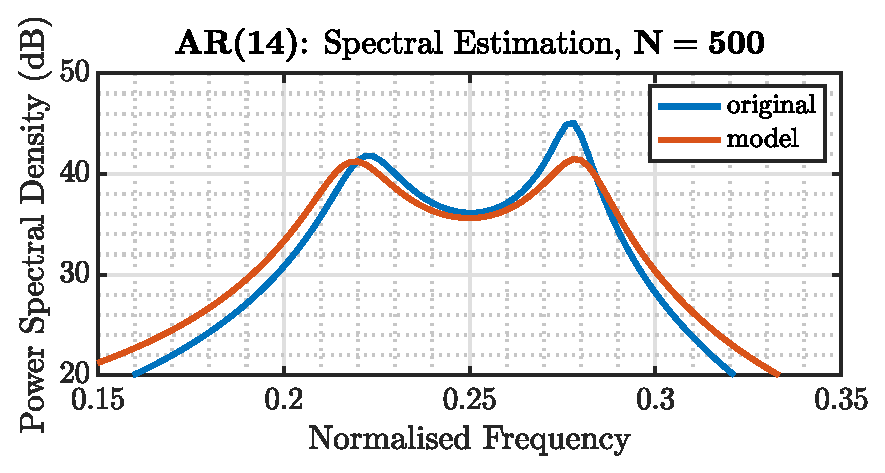
\includegraphics[height=1.5in]{report/parametric-and-line-spectra/spectrum-of-autoregressive-processes/assets/b/ar_14}
    \end{subfigure}
    \caption{AR: spectrum estimates and model order $p$ with $N=500$ samples.}
    \label{fig:2_2_b_1}
\end{figure}

Intuitively, the larger the model order $p$, the more degrees of freedom available to capture the nature of the process.
In figure \ref{fig:2_2_b_2} the noise power (mean squared prediction error) is illustrated as a function of model order $p$.
Unsurprisingly, the error decreases for increasing model order though it plateaus for $p \leq 9$. As a result, to minimize model complexity and avoid fitting error (overfitting)
model order $p = 9$ is selected.

\begin{figure}[h]
    \centering
    \begin{subfigure}{0.49\textwidth}
        \centering
        \includegraphics[height=1.5in]{report/parametric-and-line-spectra/spectrum-of-autoregressive-processes/assets/b/error}
    \end{subfigure}
    ~
    \begin{subfigure}{0.49\textwidth}
        \centering
        \includegraphics[height=1.5in]{report/parametric-and-line-spectra/spectrum-of-autoregressive-processes/assets/b/aic}
    \end{subfigure}
    \caption{AR: noise power and model order $p$ with $N=500$ samples.}
    \label{fig:2_2_b_2}
\end{figure}

We also highlight that despite the fact that $p_{original} = 4$, due to the small number of available sample ($N = 500$),
when $p = 4$ is selected the fitted model performs very poorly, thus either the number of samples should be increased or a higher order model should be used instead.

%% c)
\item
%

The experiment is repeated for the same AR process, but using $N = 10000$ samples and figures \ref{fig:2_2_c_1} and \ref{fig:2_2_c_2} are obtained.
When $p < p_{original} = 4$, the model still does not have the capacity to model the process (under-modelling) while for $p > p_{original} = 4$ the error plateaus.
Despite the fact that AR(4) model identifies the two peaks, we note that AR(5) and all higher order models track spectrum much better. To avoid overfitting the noise
and preserve generalisation of the model, criteria such as the Akaike Information Criterion (AIC) or the Bayesian Information Criterion can be used to penalise higher order models.
According to the AIC, AR(4) model is selected for this experiment, agreeing with the true model order.

\begin{figure}[h]
    \centering
    \begin{subfigure}{0.49\textwidth}
        \centering
        \includegraphics[height=1.5in]{report/parametric-and-line-spectra/spectrum-of-autoregressive-processes/assets/c/ar_3}
    \end{subfigure}
    ~ 
    \begin{subfigure}{0.49\textwidth}
        \centering
        \includegraphics[height=1.5in]{report/parametric-and-line-spectra/spectrum-of-autoregressive-processes/assets/c/ar_4}
    \end{subfigure}
    ~
    ~
    \begin{subfigure}{0.49\textwidth}
        \centering
        \includegraphics[height=1.5in]{report/parametric-and-line-spectra/spectrum-of-autoregressive-processes/assets/c/ar_5}
    \end{subfigure}
    ~
    \begin{subfigure}{0.49\textwidth}
        \centering
        \includegraphics[height=1.5in]{report/parametric-and-line-spectra/spectrum-of-autoregressive-processes/assets/c/ar_9}
    \end{subfigure}
    \caption{AR: spectrum estimates and model order $p$ with $N=10000$ samples.}
    \label{fig:2_2_c_1}
\end{figure}

\begin{figure}[h]
    \centering
    \begin{subfigure}{0.49\textwidth}
        \centering
        \includegraphics[height=1.5in]{report/parametric-and-line-spectra/spectrum-of-autoregressive-processes/assets/c/error}
    \end{subfigure}
    ~
    \begin{subfigure}{0.49\textwidth}
        \centering
        \includegraphics[height=1.5in]{report/parametric-and-line-spectra/spectrum-of-autoregressive-processes/assets/c/aic}
    \end{subfigure}
    \caption{AR: soise power and model order $p$ with $N=10000$ samples.}
    \label{fig:2_2_c_2}
\end{figure}

%
\end{enumerate}